\documentclass[twocolumn,superscriptaddress,aps,prb,floatfix]{revtex4-1}

\usepackage{graphicx}% Include figure files
\usepackage{dcolumn}% Align table columns on decimal point
\usepackage{bm}% bold math
\usepackage{color}
\usepackage[caption=false]{subfig} 

\usepackage{listings}
\usepackage{cancel}

\definecolor{dkgreen}{rgb}{0,0.6,0}
\definecolor{gray}{rgb}{0.5,0.5,0.5}
\definecolor{mauve}{rgb}{0.58,0,0.82}

\lstset{frame=tb,
  language=python,
  aboveskip=3mm,
  belowskip=3mm,
  showstringspaces=false,
  columns=flexible,
  basicstyle={\small\ttfamily},
  numbers=none,
  numberstyle=\tiny\color{gray},
  keywordstyle=\color{blue},
  commentstyle=\color{dkgreen},
  stringstyle=\color{mauve},
  breaklines=true,
  breakatwhitespace=true,
  tabsize=3
}

\usepackage{amsthm}
\usepackage{amsmath}
\usepackage{amssymb}

\newcommand{\Htc}{H_{\mathrm{TC}}}
\newcommand{\Hising}{H_{\mathrm{Ising}}}
\newcommand{\figref}[1]{Fig. \ref{#1}}


\newcommand{\blue}[1]{{\color{blue} { #1}}}
\newcommand{\red}[1]{{\color{red} { #1}}}
\newcommand{\green}[1]{{\color{green} { #1}}}
\newcommand{\needcite}{{\color{blue} {[Citation needed]}}}

\newtheorem{theorem}{Theorem}[section]
\newtheorem{lemma}[theorem]{Lemma}
\newtheorem{proposition}[theorem]{Proposition}
\newtheorem{corollary}[theorem]{Corollary}

%\newenvironment{proof}[1][Proof]{\begin{trivlist}
%\item[\hskip \labelsep {\bfseries #1}]}{\end{trivlist}}
%\newenvironment{definition}[1][Definition]{\begin{trivlist}
%\item[\hskip \labelsep {\bfseries #1}]}{\end{trivlist}}
%\newenvironment{example}[1][Example]{\begin{trivlist}
%\item[\hskip \labelsep {\bfseries #1}]}{\end{trivlist}}
%\newenvironment{remark}[1][Remark]{\begin{trivlist}
%\item[\hskip \labelsep {\bfseries #1}]}{\end{trivlist}}

%\newcommand{\qed}{\nobreak \ifvmode \relax \else
%      \ifdim\lastskip<1.5em \hskip-\lastskip
%      \hskip1.5em plus0em minus0.5em \fi \nobreak
%      \vrule height0.75em width0.5em depth0.25em\fi}

\begin{document}

%\allowdisplaybreaks

\title{Stable quantum memories with few measurements}
%\title{Finite temperature thresholds for stabilizer codes with few measurements}


\author{C. Daniel Freeman}
\email{daniel.freeman@berkeley.edu}
\affiliation{Berkeley Quantum Information \& Computation Center, University of California, Berkeley, CA 94720, USA}
\affiliation{Department of Physics, University of California, Berkeley, CA 94720, USA}

\author{Mohan Sarovar}
\email{mnsarov@sandia.gov}
\affiliation{Sandia National Laboratories, Livermore, CA}

\author{C. M. Herdman}
\affiliation{Institute for Quantum Computing, University of Waterloo, Waterloo, ON N2L 3G1, Canada}
\affiliation{Department of Chemistry, University of Waterloo, Waterloo, ON N2L 3G1, Canada}
\affiliation{Department of Physics \& Astronomy, University of Waterloo, Waterloo, ON N2L 3G1, Canada}

\author{K. B. Whaley}
\affiliation{Berkeley Quantum Information \& Computation Center, University of California, Berkeley, CA 94720, USA}
\affiliation{Department of Chemistry, University of California, Berkeley, CA 94720, USA}

\date{\today}

\begin{abstract}
 We demonstrate the existence of a finite temperature threshold for a 1D stabilizer code under an error correcting protocol that uses only a fixed, constant fraction of the syndrome measurements.  We sketch how this algorithm generalizes to higher dimensional stabilizer codes with string-like excitations, like the toric code. 
\end{abstract}

\maketitle

%%%%%%%%%%%%%%%%%%%%%%
%%%%%%%%%%%%%%%%%%%%%%
\section{Introduction}
\label{sec:Intro}
%%%%%%%%%%%%%%%%%%%%%%

Quantum memories are an essential component for many quantum technologies, including quantum computing and quantum repeaters. In analogy to modern classical memories, one ideally wants a stable quantum memory that requires little or no active intervention and error correction. Unfortunately, no physical system that passively preserves quantum information indefinitely at finite temperatures and in an experimentally accessible number of dimensions is known \cite{Terhal:2015ks}. Instead, the operation of all known practical quantum memories require a combination of passive elements (i.e. dissipative cooling) and active measurement and correction cycles to keep quantum information protected.  In this work, we study the degree to which the amount of active measurement and correction can be reduced while maintaining quantum memory stability (our notion of stability, to be quantified later, corresponds to exponentially long lifetime for encoded states at some finite threshold temperature). We develop a new decoding and correction protocol that enables one to trim the number of measurements to a fraction of the complete set of measurements normally considered, and still maintain quantum memory stability. 

We restrict our attention to quantum memories defined through stabilizer codes. For near term architectures, stabilizer codes\cite{Gottesman98} have emerged as the leading candidate for encoding quantum information and subsequent active error correction in quantum hardware, with small scale architectures actively being developed and deployed\cite{all the stabilizers}. \red{A tremendous amount of effort has gone into developing novel decoding schemes for stabilizer codes.  Cite Adrian Hutter, Harrington, Others.  More Background.}
 
 In previous work \cite{Freeman2014}, we analyzed the finite temperature dynamics of the toric code, verifying the well-known no-go theorems for the upper bound to the lifetime of the toric code at finite temperature \needcite.  Using this analysis, we were able to construct a measurement-free protocol for protecting the encoded qubits of the toric code \cite{Freeman2016}, but these protocols again were limited by the no-go theorems, and only provided a multiplicative constant increase to the lifetime.  
 
Building off this previous work, here we examine the extent to which a limited amount of measurement can increase the lifetime of stabilizer codes with string-like excitations.  In sum, we demonstrate an algorithm that, for any constant density of measurements for a stabilizer code with stringlike excitations undergoing dissipation at a fixed temperature, a threshold can be achieved.  The threshold temperature scales with the amount of measurement used---fewer measurements result in a smaller threshold temperature, whereas more complete measurement raises the threshold temperature.  This tradeoff is commensurate with and complements what is known about decoding the stabilizer codes in the presence of \emph{noisy}, but complete measurements.
 
 The remainder of the manuscript is structured as follows:  Section \ref{sec:stabfintemp} briefly reviews the theoretical tools used for performing simulation of stabilizer codes at finite temperature.  The content of this section is also expanded upon in refs \cite{Freeman2014,Freeman2016}.  Section \ref{sec:ecc_alg} includes the full description of our few-measurement algorithm, including a discussion of the expected low temperature error processes that cause the algorithm to fail, and a heuristic justification for the expectation of a threshold at low temperature.  Section \ref{sec:experiments} details our numerical investigations of our algorithm for the 1D Ising model.  Finally, Sec. \ref{sec:tc_alg} sketches how this algorithm could be generalized to higher dimensions, and Sec. \ref{sec:discussion} provides some concluding analysis and discussion.
 
 
 
 
%%%%%%%%%%%%%%%%%%%%%%
\section{Stabilizer codes at Finite Temperature}
\label{sec:stabfintemp}

\subsection{Definitions}
\label{sec:Defs}
%%%%%%%%%%%%%%%%%%%%%%
In this section, we briefly review the theory of the 1D Ising model, as well as the Markovian open quantum systems formalism for evaluating its finite temperature dynamics.  The Hamiltonian for the 1D Ising model is

\begin{align}
\Hising = -\Delta \Sigma_i \sigma^i_z \sigma^{i+1}_z
\label{eq:isingham}
\end{align}

where, for the remainder of the manuscript, unless explicitly stated otherwise, we assume $\Delta=1$.  This also fixes our units for temperature.  This is exactly the Hamiltonian version of the repetition stabilizer \emph{code}\cite{Freeman2016}.  Note that the terms $\sigma^i_z \sigma^{i+1}_z$ exactly correspond to the parity check stabilizer operators of the repetition code.  Confer with Table \ref{tab:code_vs_hamiltonian} for the correspondences between the stabilizer Hamiltonian and stabilizer code versions of the 1d Ising model.

\begin{table}
\begin{center}
  \begin{tabular}{ l | r }
    \hline
    Repetition Stabilizer Code & 1d Ising Stabilizer Hamiltonian \\ \hline
    Encoded States & Ground States \\ \hline
    Bit flip errors & Excited States \\ \hline
    Error correction via decoder & Same or via cooling \\ \hline
    \hline
  \end{tabular}
\end{center}
\caption{A short summary of the similarities and differences between the Ising model considered as a code versus as a hamiltonian.}
\label{tab:code_vs_hamiltonian}
\end{table}

In the parlance of the 1D Ising model, bit flip errors are often also classified via the dual variables called \emph{domain walls}.  Domain walls are simply locations on the 1D Ising chain where a stabilizer operator yields a measurement of $-1$---i.e., locations where neighboring spins point in different directions.  With periodic boundary, the number of these locations is always a multiple of two, and a single bit flip event either creates a pair of such domain walls, deletes a pair of domain walls, or causes a domain wall to translate by one unit.  

Whether considered as a code or as a Hamiltonian, the condition for whether a state of the system with errors present can be reliably returned to an encoded state is the same: so long as less than half the system has had errors, a majority rule decoder that has access to measurements of the full set of stabilizers ${\sigma^i_z \sigma^{i+1}_z}$ will reliably be able to correctly remove errors.  When errors are completely independent (i.e., at very high temperature), we can define random variables $x_i=1$ when an error occurs on site $i$, and $0$ otherwise.  If these errors occur with probability $p$ on each spin, independently at random every error detection cycle, then Chernoff's bound gives an upper bound to the probability of an error in the encoded space, $P(\Sigma_i x_i \geq L/2) \leq \rm{exp}[-Lp\frac{\delta^2}{2+\delta}]$ for $\delta=1/2p-1$.  Thus, for complete measurement, errors in the encoded subspace are exponentially suppressed in system size, so long as the error rate is sufficiently small.

For much of the remainder of the manuscript, we consider how the decoding scheme changes when one does \emph{not} have access to the full set of stabilizer measurements.

Following \ref{Freeman2016}, we consider a simple local Ohmic, Markovian bath to model finite temperature effects.  This is modeled by the following master equation in Lindblad form:

\begin{align}
\dot{\rho }=\sum_{\omega }{2c_{\omega }\rho c^{\dagger }_\omega}-c^{\dagger }_{\omega }c_{\omega }\rho -\rho c^{\dagger }_{\omega }c_{\omega }, \label{eq:Lindblad}
\end{align}

for the density matrix $\rho$, with Lindblad operators $c_{\omega }$ chosen to take the form:

\begin{equation}
\left \{ c_\omega \right \} = \left \{ \sqrt{\gamma(0)} T_{b}, \sqrt{\gamma(1)} D^\dagger_{b}, \sqrt{\gamma(-1)} D_{b} \right\} 
\end{equation}
where $D_{b}$ dissipates a pair of domain walls,  $D^\dagger_{b}$ creates a pair of domain walls, $T_{b}$ translates a domain wall by one unit, and $\gamma(\cdot)$ is a rate function dependent on the details of the bath.  This bath is chosen to model the dynamics of local, single bit-flip errors.  In the Pauli basis, these operators take the following form.

\begin{align}
D^\dagger_{b}= &\frac{1}{4} \left(I \sigma_x I \right)\left(1+I \sigma_z \sigma_z\right)\left(1+ \sigma_z \sigma_z I\right) \notag \\
D_{b}= &\frac{1}{4} \left(I \sigma_x I \right)\left(1-I \sigma_z \sigma_z\right)\left(1-\sigma_z \sigma_z I\right) \notag \\
T_{b}= &\frac{1}{4} \left(I \sigma_x I \right)\left(1-I \sigma_z \sigma_z\right)\left(1+ \sigma_z \sigma_z I\right) \label{eq:LindbladDef}
\end{align}

Finally, the remaining details of the bath are specified by the spectral density, which determines the rates with which the different Lindblad operators act:

\begin{align}
\gamma \left( \omega \right)=\xi \left  \vert \frac{\omega^n }{1-e^{-\beta \omega }} \right \vert \label{eq:gammadef}
\end{align}

Choosing $n=1$ corresponds to an Ohmic spectral density, which is the choice we make for the remainder of the manuscript.  With this choice, in the absence of any error correcting protocol, the 1D Ising model has a system size independent thermal error rate given by\cite{Freeman2016}

\begin{align}
\Gamma_0 = \frac{\gamma(0)}{1+e^{1/T}} 
\end{align}

We define its bare lifetime to be $\Gamma_0^{-1}$.

\subsection{Finite Temperature vs. Infinite Temperature}
\label{sec:temperature}

 The vast majority of the error correction literature assumes an error model akin to an ``infinite temperature limit''.  More precisely, an array of qubits receives errors from some set of error operators ${E_i}$ independently at random with some probability $p$ every error correction cycle.  The threshold theorems state that there exists some critical error probability $p_c$ below which it is possible to return an error correcting code to its encoded state with unit probability for asymptotically large systems.  For the toric code, $p_c\approx.11$.
 
 Contrariwise, thresholds at finite temperature are usually quoted in terms of a critical \emph{temperature}.  That is, there must exist some critical temperature $T_c$ below which codes can be reliably corrected.  Unfortunately, this definition obscures a great deal of physics---different choices of bath model can greatly affect the dynamics of the error processes, to the extent that a quoted ``critical temperature'' often implicitly specifies a choice of bath model.  Because different bath interactions can give rise to different system dynamics, the choice of bath also directly affects the strategy used for error correction.  For example, it is known that the toric code's threshold temperature is altered by considering a correlated bath \red{time or space correlated?} rather than an uncorrelated one \cite{Novais13}.
 
 The main consequence of choosing an Ohmic bath is that it sets the amplitude of the excitation hopping process.  That is, $\gamma(0)$ is determined by the $\omega \rightarrow 0$ limit of the spectral density of the bath, and for the Ohmic bath taking the $\omega\rightarrow0$ limit of  Eq. \ref{eq:gammadef} yields $\gamma(0) \sim T$. 
Ultimately, this means that the hopping rate of domains walls is controlled by this choice of bath model. At finite temperatures, this introduces correlations into the patterns of errors that effect the system, and so it is no longer possible to talk about an ``independent error probability per site''. 
In contrast to the behavior of $\gamma(0)$, 
the other operationally important feature of the bath, the ratio of domain wall creation and annihilation rates, is set by detailed balance to Boltzmann-like scaling (i.e., $\gamma(1)/\gamma(-1) = \exp(-1/T)$), and is independent of the choice of bath spectrum.   
 
 In the most extreme case, at sufficiently low temperature, errors are most often immediately dissipated by the bath upon creation.  However, because domain walls that are not immediately adjacent cannot be dissipated by the bath, the system occasionally becomes ``trapped'' in the first excited state by a rare pair creation followed by pair hopping event -- i.e., a $D^\dagger_{b}$ followed by a $T_{b}$ -- before the bath can dissipate the excitation.  Then any subsequent errors are overwhelmingly more likely to act on existing pair of domain walls, translating them around in a one-dimensional random walk.
 
 Thus, error correction for the 1D Ising model at low temperature with this sort of bath dynamics is equivalent to attempting to identify these randomly-migrating rare pairs of domain walls.  While a majority-rule decoding scheme works in both low and high temperature limits for the Ising model, if the number of measurement resources is restricted, the standard majority rule scheme breaks down.  
 


 
  %%%%%%%%%%%%%%%%%%%%%%
%%%%%%%%%%%%%%%%%%%%%%
\section{Few Measurement Error Correction Algorithm}
\label{sec:ecc_alg}
%%%%%%%%%%%%%%%%%%%%%%

\subsection{The Algorithm}

In this section, we sketch a new algorithm which reliably dissipates defects in the 1D Ising model below a threshold temperature, which we determine numerically.  The primary technical innovation of this algorithm, and its generalization to quantum memories based on any stabilizer Hamiltonian, is that it does not require measurement of the complete set of stabilizer operators for a given stabilizer code---only a fixed subset.  We assume that the system is subject to periodic measurements on periodically spaced measurement ``patches'', that measurement readout and processing occurs much faster than any system timescale, and that the system is subject to a thermal bath as described in Sec. \ref{sec:Defs}.

\begin{figure}
\begin{center}
\scalebox{1}{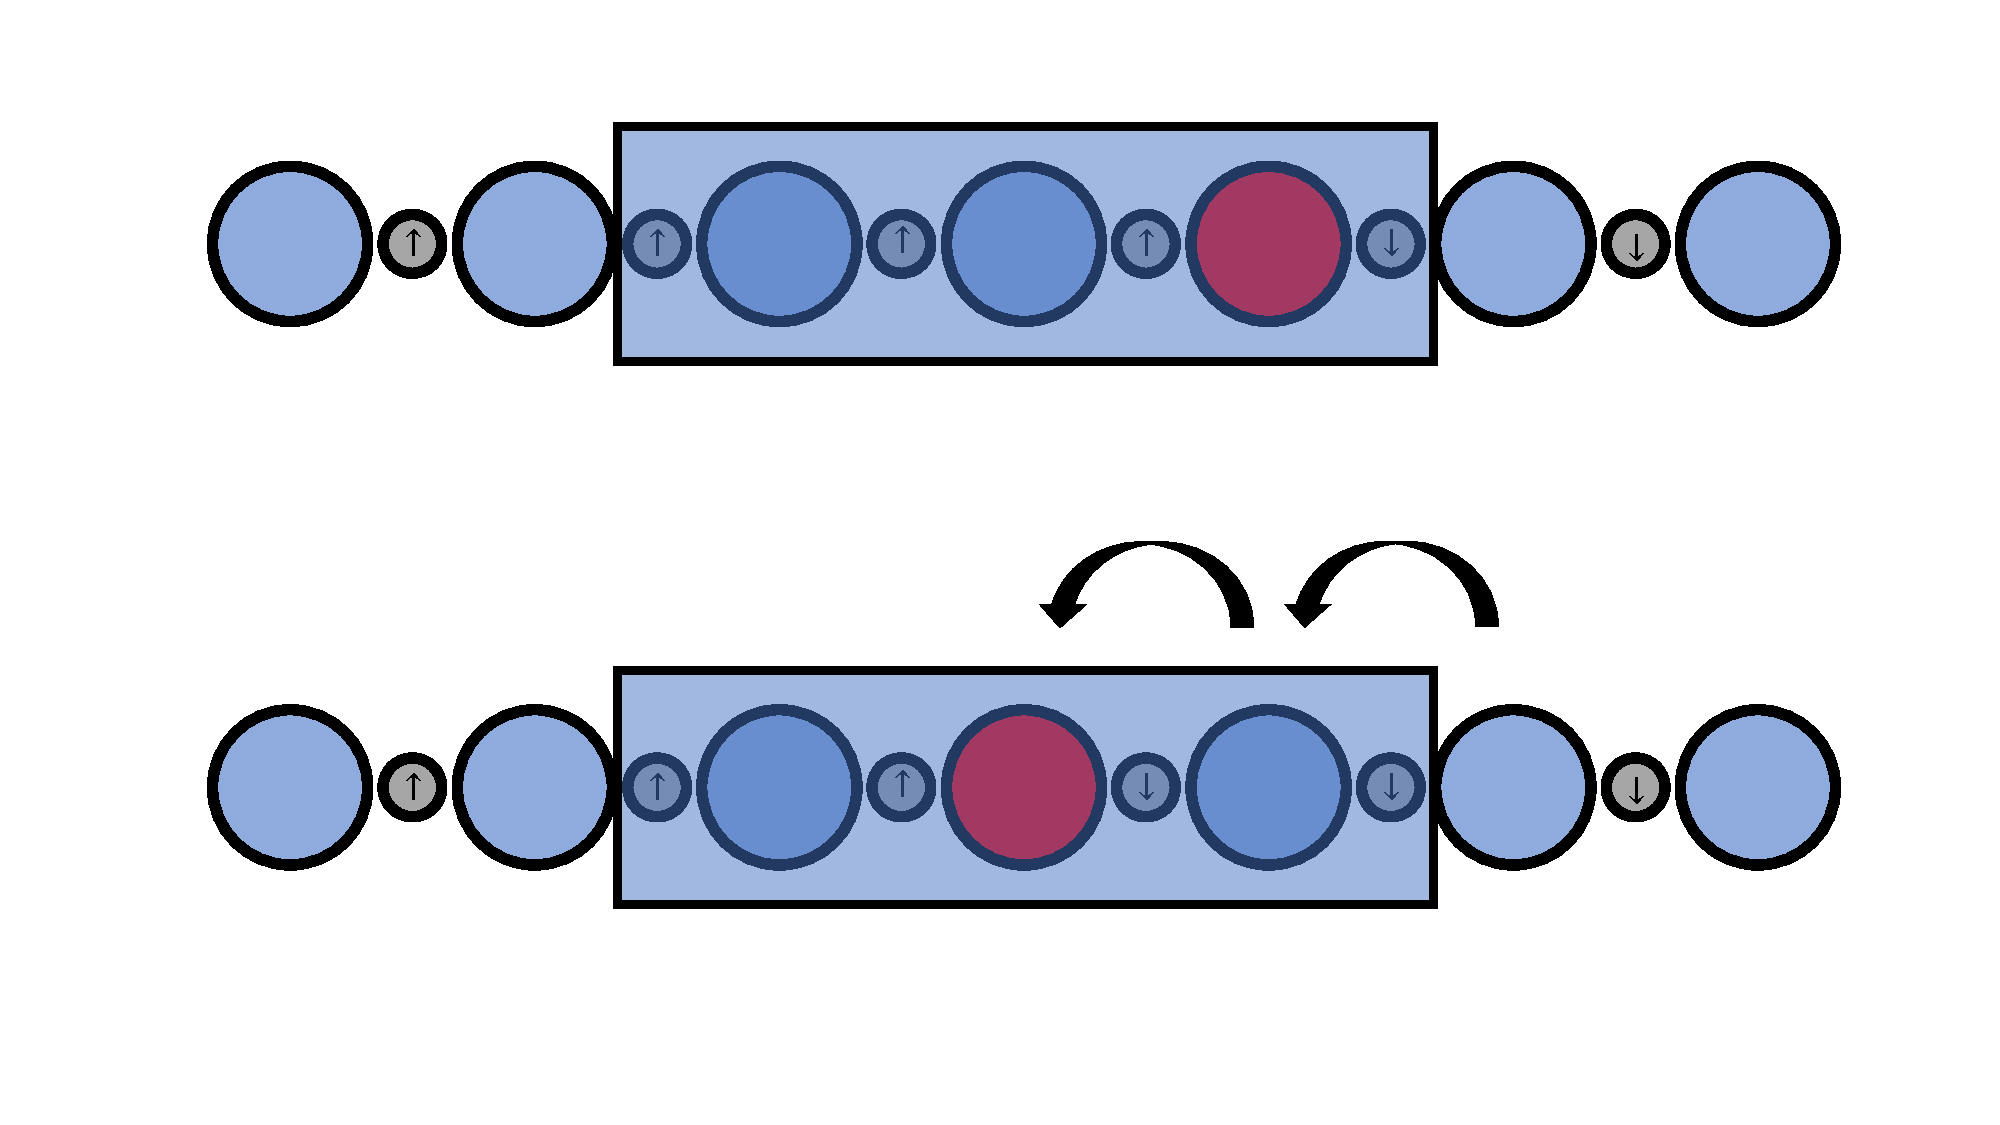
\includegraphics[width=1.0\columnwidth]{detect_swap.pdf}}
\end{center}
\caption{This cartoon illustrates the ``centering'' procedure for detected defects.  Spin variables are in gray, and domain wall variables are in blue (no defect present) and red (defect present).  When a defect is detected on a measurement patch (blue box), it is swapped to the center of the measurement patch via the $\rm{DSWAP}$ operator (black arrows).  The defect immediately adjacent to it is also swapped onto the measurement patch so as not to pull apart defect pairs that would have otherwise dissipated.}
\label{fig:detect_swap}
\end{figure}

The algorithm can be summarized in fives steps:

1. Measure stabilizers on patches, keeping record of the age of defects that are already on patches, as well as defect locations.

2. Perform ``centering'' on patches with defects (see \figref{fig:detect_swap}), based on centering protocol introduced in Ref. \cite{Freeman2016}.

3. Calculate probability of fusion (explicitly given in Eq. \ref{eq:bayes_simple}) for all pairs of measured defects residing on the measurement sites.

4. Probabilistically perform error correction based on probabilities calculated in step 3.

5. Repeat

Step 2 encourages defects to remain localized at measurement patches.  This centering protocol can be performed entirely unitarily by the $DSWAP$ operator, which takes the following form in the Pauli basis,
\begin{align}
\rm{DSWAP} &= \frac{1}{2} \left(III + I\sigma_x I + \sigma_z I \sigma_z - \sigma_z \sigma_x \sigma_z \right)
\end{align}

The centering process aids the probability of fusion calculation by ensuring that the coordinates and measurement times are representative of when and where defects are actually created.  If defects escape from measurement patches, then upon being measured again, the time recorded by the measurement patch now underestimates how old the defect actually is, biasing the probability estimate.  This centering operation greatly reduces the probability of defect escape.

 Note that the pattern of $\rm{DSWAP}s$ used in \figref{fig:detect_swap} also swaps the neighboring, \emph{unmeasured} defect onto the measurement patch.  This is to ensure that the protocol does not inadvertently create a new separated pair of domain walls in the system by shifting only one domain wall in a potentially adjacent pair. 
 
\subsection{Fusion Probability Calculation}
\label{sec:bayes_prob_calc}

%************************TRIM SUBSTANTIALLY AND PUT IN APPENDIX

To perform error correction properly, we need to be able to estimate the probability that two given measured defects are a pair, given that they have been measured at two particular measurement patches at two different times.  For notational convenience, we define:
\begin{align}
d_1 : d_2 \equiv {\rm defect}\ d_1\ {\rm and}\ d_2\ {\rm are\ a\ pair}
\end{align}
and
\begin{align}
d_i^{x_1,t_1} \equiv {\rm defect}\ d_i\ {\rm measured\ at\ time}\ t_1\ {\rm at\ patch}\ x_1
\end{align}

Then, we aim to calculate the fusion probaility:
\begin{align}
P(d_1:d_2 | d_1^{x_1,t_1} \wedge d_2^{x_2,t_2}),
\end{align}
i.e., the probability that two detects measured at spacetime coordinates $(x_1,t_1)$ and $(x_2,t_2)$ are part of the same defect pair, and therefore should be fused in a correction step.

To calculate this probability, we proceed via Bayes rule: 
\begin{align}
\label{eq:bayes}
&P(d_1:d_2 | d_1^{x_1,t_1} \wedge d_2^{x_2,t_2}) = \\ \notag
&\frac{P(d_1^{x_1,t_1} \wedge d_2^{x_2,t_2} | d_1:d_2) P(d_1 : d_2)}{P(d_1^{x_1,t_1}\wedge d_2^{x_2,t_2})}
\end{align}
The individual terms on the right hand side of equation \ref{eq:bayes} are straightforward to interpret.  $P(d_1^{x_1,t_1} \wedge d_2^{x_2,t_2} | d_1:d_2)$ represents the probability that two measured defects would be at $(x_1,t_1)$ and $(x_2,t_2)$ given that they are indeed a pair.  This can be related to the probability that a one dimensional diffusion process with diffusion constant $D$ will perform an excursion of distance $|x_2-x_1|$ or greater in a time $t_2 - t_1$; \textit{i.e.,} will perform an excursion that can measurement patches at $x_1$ and $x_2$. Explicitly,
\begin{align}
\label{eq:bayesformula}
&P(d_1^{x_1,t_1} \wedge d_2^{x_2,t_2} | d_1:d_2) \\ \notag
&= 1-2\int_{0}^{|x_2-x_1|} dx \frac{1}{2\pi D |t_2-t_1|} \rm{exp}\bigg(-\frac{|x_2-x_1|^2}{2 D |t_2-t_1|}\bigg) \\ \notag 
&= 1 - {\rm erf}\bigg(\frac{|x_2-x_1|}{2\sqrt{D |t_2 - t_1|}}\bigg) 
\end{align}
For our analysis, we will choose $D\propto \gamma_0$.  The exact correspondence between $D$ and $\gamma_0$ depends on the details of the error correction algorithm itself, so, in practice, we treat the constant of proportionality as an empirically tuned parameter.  Furthermore, we approximate any detected defects as arising from a pair that was created an equal distance between the measurement patches at locations $x_1$ and $x_2$ for the purposes of calculating the probability in Eq. \ref{eq:bayesformula}.

$P(d_1 : d_2)$ represents the probability that two measured defects, $d_1$ and $d_2$, are in fact a pair.  Finally, $P(d_1^{x_1,t_1}\wedge d_2^{x_2,t_2})$ is the probability that two defects are measured, one at $(x_1,t_1)$, and the other at $(x_2,t_2)$.  As we discuss in Appendix \ref{sec:bayesdecoder}, these factors are not as important for the decoding scheme as Eq. \ref{eq:bayesformula}.  In practice, we find that using the expression from Eq. \ref{eq:bayesformula} alone is sufficient to provide resilient error correction.  We defer further discussion to the appendix.
 
 
 \subsection{Common error modes and analysis}
 \label{sec:threshold}
 
 The two primary failure modes of the error correction procedure are (1) defects escaping measurement patches, and (2) defects being paired incorrectly. These failure modes become more harmful as temperature increases.  Failure mode 1 can be suppressed by working with large measurement patches, as the escape timescale is exponential in the number of sites within the measurement patch---i.e., it scales like $(1/\gamma_0)^{\rm{\#\ of\ sites\ on\ patch}}$.  Failure mode 2 can be suppressed to a degree, but at high enough temperature, will eventually happen with high probability, as is the case in the full-measurement version of the protocol.  If too many errors are introduced between measurement cycles, it becomes impossible to correct the system even in principle because the syndrome measurements can no longer be unambiguously decoded.  At sufficiently low temperature, however, with some assumptions, our algorithm can extend the lifetime of the system exponentially in system size.
 
 Suppose that (a) defects are efficiently trapped by the measurement patches, and (b) temperature is low so that there is $\rho \ll 1$ defect pair per measurement patch.  In this regime, condition (a) guarantees that defects do not escape measurement patches.  Then, the only error pathway is a sequence of incorrect, but nonetheless ``plausible'' error correction operations, whereby some sdefects are paired with defects that are not their own pair.  
%************************Make explicit here that it's a heuristic argument.  Because the error processes in our model are difficult to etc. etc. etc.
 To upper bound this error rate, note that such erroneous pairing occurs because one member of a paired defect has not yet been measured.  In other words, one defect of a pair is measured, and the other defect spends ``too long'' migrating around in the unmeasured bulk region.  Suppose that the average amount of time a defect spends sitting on a measurement patch is $\tau_s$, and the average time it takes a defect to be detected on a measurement patch, after creation, is $\tau_d$.  Further suppose $\tau_s/\tau_d = \delta \ll 1$---that is, on average, defects are unlikely to escape from a measurement patch over the timescale it takes a defect to migrate within the bulk region to a measurement patch.

 Treating the full dynamics of errors is difficult, so we first consider a different, simpler error dynamics.  First, we argue how, in the presence of this simpler error model, our algorithm provides an exponentially long lifetime in system size.  Then, we argue how this simpler error model is actually more pessimistic with respect to possible error processes than the true error dynamics---that is, we expect the real model to have a \emph{better} lifetime scaling than would be expected from the simple error model.
 
 The simple error model is defined as follows:  suppose that a single pair of defects is in a system, and that no new pairs will be introduced.  One of the pair is fixed on a measurement rail, and the other is, at time 0, undetected.  Further, suppose that there is an error process that occasionally translates the unmeasured defect by an amount $2\sqrt{\gamma_0 \delta t}$, for hopping rate $\gamma_0$ and for system time $\delta t$.  Note that this means the error process acts on longer distance scales as system time increases.  The particular form of this error process is chosen to mimic a spurious error correction event, where a pair of defects is ``corrected'', but this pair of defects was not a real pair, leaving another unmeasured defect even further away.  As time increases, the characteristic distance over which this error process could occur also increases, in accordance with the typical pair-wise separation between two defects performing a random walk.  This typical distance is exactly the factor used by the error correction algorithm to determine if a pair of defects should be corrected or not.  Thus, the error process is representative of a worst case error correction event that not only pairs the wrong two defects, but leaves the system in a configuration with an unmeasured defect as far separated from the measured defect as possible.

 If this error process happens every $\tau_{\epsilon}$, then an uncorrectable error will occur if the bulk defect remains undetected up until it crosses half the system.  For patches of size $\lambda$, the probability that this occurs is roughly $(\tau_{\epsilon} / \tau_d)^{k}$, where $k$ is the number of times the error process must occur for the error process to have separated the defects a distance $(L/2\lambda)$ and $\tau_d$ is the timescale associated with a non-erroneous error correction operation.  Because this error process happens approximately every $\tau_{\epsilon}$, after a timescale $q*\tau_{\epsilon}$, the defect pairs will have been separated a distance $\Sigma^q_{i=1} \sqrt{i * \gamma_0 \tau_{\epsilon}}$, assuming that they are never correctly paired.  This sum $\Sigma^q_{i=1} \sqrt{i}$ grows asymptotically like $q^{3/2}$.  Thus, $k$ then scales approximately like $(L/\lambda)^{2/3}$.
 
 Finally, if we have $L/\lambda$ such simultaneous error processes independently in the system---one for each measurement patch---then the total error probability scales like
\begin{align}
\label{eq:err_scaling}
 P(\rm{uncorrectable\ error}) \leq (L/\lambda) (\tau_{\epsilon} / \tau_d)^{(L/\lambda)^{2/3}}.
\end{align}

For this system, $\tau_{\epsilon}$ is much smaller than $\tau_d$, thus the full probability of erroneous corrective operations is exponentially small in system size.
 
 This probability serves as an upper bound because it is extremely pessimistic about the sorts of error processes occurring.  Note that in the real system, a spurious error correction process that effectively increases the distance between a pair of defects also reduces the total number of defects by two.  Thus, while our toy error model is ``non-interacting''---that is, it assumes $L/\lambda$ independent error processes which, in sum, take the form described in Eq. \ref{eq:err_scaling}---a more careful treatment of the error process, including interactions between defects, as in the real model, would result in an error probability \emph{smaller} than the one calculated here.
 
 In the following section, we provide numerical evidence that the lifetime of the Ising model in the presence of the protocol scales quasi-exponentially with the number of measurement patches, as anticipated by the upper bound in Eq.\ref{eq:err_scaling}.
 

 
 %%%%%%%%%%%%%%%%%%%%%%
%%%%%%%%%%%%%%%%%%%%%%
\section{Finite Temperature Simulations}
\label{sec:experiments}
%%%%%%%%%%%%%%%%%%%%%%

In this section, we examine the behaviour of the protocol at different system sizes, temperatures, and measurement fractions.  While data is reported in terms of system size, the more fundamental length scale is the characteristic size of the \emph{measurement patch}.  This is because the size of the measurement patch is the shortest length scale relevant to the algorithm, and thus controls the majority of the scaling behavior.  Perhaps unsurprisingly, systems of radically different size but with the same number of measurement patches have fairly comparable lifetimes (e.g., size 200 system with 10 patches versus size 100 system with 10 patches).  We elaborate on the scaling of the measurement fractions further in the discussion.  Unless otherwise noted, the data reported here are for systems with 3 measured sites for every 7 sites for a measurement fraction of $3/7$.  Thus, the total size of unit cell is $\lambda=7$, there are $\lambda_m=3$ measured sites, and $\lambda_b=4$ bulk sites, as is depicted in Fig. \ref{fig:detect_swap}.

\begin{figure}
\begin{center}
\scalebox{1}{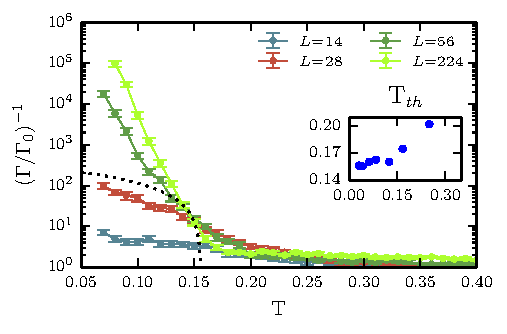
\includegraphics[width=1.0\columnwidth]{LifetimeVsTemperature.pdf}}
\end{center}
\caption{Lifetime of various system sizes as a function of temperature.  Measurement fraction is $3/7$.  Notice the transition between no-effect, and significant lifetime improvement near $T=.16$.  A $3/7$ measurement fraction was used for this data.}
\label{fig:LifetimeVsTemperature}
\end{figure}

\figref{fig:LifetimeVsTemperature} depicts the scaling of the system lifetime with temperature.  At low temperatures, the system lifetime increases dramatically with both lower temperatures, and larger system size.  Due to finite size effects, it is difficult to extract an unambiguous threshold temperature, but below $T\approx.13$, the lifetime manifestly increases with larger system size.  We empirically define a threshold temperature by the choosing a large system size, fitting a curve to the Lifetime versus Temperature data which results in a lifetime improvement greater than a factor of $10$, and then back-extrapolating where this curve crosses the Temperature axis.

\begin{figure}
\begin{center}
\scalebox{1}{\includegraphics[width=1.0\columnwidth]{LifetimeVsSystemSize.pdf}}
\end{center}
\caption{Lifetime of the Ising model at various temperatures plotted against system size.  Note the monotonic growth in lifetime for low temperature models, as well as the plateau in lifetime for moderately sized systems. A $3/7$ measurement fraction was used for this data.}
\label{fig:LifetimeVsSystemSize}
\end{figure}

This is clearer in \figref{fig:LifetimeVsSystemSize}, which depicts the scaling of the lifetime with system size directly.  Note that, for models above $T\approx.13$, larger system sizes asymptote to a fixed lifetime improvement, whereas for models below $T\approx.13$, the lifetime grows quasimonotonically with system size.  Beyond $L=100 (\lambda\approx15)$, finite size effects are significantly reduced.  This is because small-system sizes cannot easily suppress second order errors, such as defects escaping from measurement patches or multiple pairs of defects in the system.  Such errors are actually uncorrectable for systems of charateristic size $\lambda\leq4$ $(L=28$ for plotted data$)$---hence the plateau appearing around $L=50 (\lambda=7)$ to $L=100 (\lambda=12)$.  This plateau is of height $O((\Gamma_0^2)^{-1})$---the characteristic timescale of these ``second-order'' events.  This scaling is more clear when plotting the liftime divided by the bare lifetime squared---i.e. $\Gamma / \Gamma_0^2$---as in \figref{fig:LifetimeVsSystemSizeReduced}.

%************************PUT IN TERMS OF SYSTEM SIZE
%************************MAYBE REMOVE INTERMEDIATE SYSTEM SIZES - remove 12,16,24 from Fig. 2 or maybe just 4,8,16,32.
%************************Mush together figure 3 and 4 maybe?
%************************Lines in fig. 5 and fig. 7 to guide the eye
%************************include m and system sizes in figure captions
%************************maybe have a plot for Delta critical temperature scaling
%************************make the toric code figure sparser perhaps?

\begin{figure}
\begin{center}
\scalebox{1}{\includegraphics[width=1.0\columnwidth]{LifetimeVsSystemSizeReduced.pdf}}
\end{center}
\caption{The same data in \figref{fig:LifetimeVsSystemSize} rescaled by an additional factor $\Gamma_0^{-1}$, to emphasize the origin and scaling of the plateau in system lifetimes.}
\label{fig:LifetimeVsSystemSizeReduced}
\end{figure}

\begin{figure}
\begin{center}
\scalebox{1}{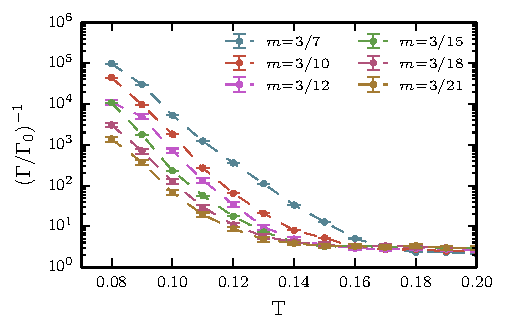
\includegraphics[width=1.0\columnwidth]{LifetimeVsMeasurementFraction.pdf}}
\end{center}
\caption{Several measurement fractions plotted as a function of temperature at fixed number of measurement patches.  Note the shift in the threshold temperature as a function of measurement fraction.}
\label{fig:LifetimeVsMeasurementFraction}
\end{figure}

Another free parameter in the algorithm is the ratio of measured sites $\lambda_m$ to bulk sites $\lambda_b$.  For this work, we fixed $\lambda_m=3$ and varied $\lambda_b$.  \figref{fig:LifetimeVsMeasurementFraction} depicts the effect measuring fewer sites on the system lifetime as a function of temperature for several different measurement fractions.  In sum, measuring a smaller fraction of the lattice causes the threshold temperature to shift downwards.  This scaling of the threshold temperature itself is depicted explicitly in \figref{fig:CriticalTempVsMeasurementFraction}.

\begin{figure}
\begin{center}
\scalebox{1}{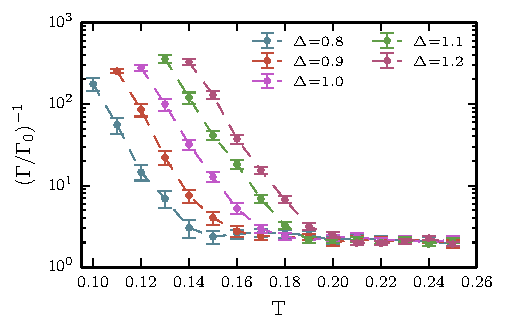
\includegraphics[width=1.0\columnwidth]{LifetimeVsTemperatureVsEnergy.pdf}}
\end{center}
\caption{Here we plot the lifetime of the system as a function of temperature for a variety of energy scales $\Delta$ (see Eq. \ref{eq:isingham}) for an $L=224$ system.  A $3/7$ measurement fraction was used for this data.}
\label{fig:LifetimeVsTemperatureVsEnergy}
\end{figure}


%%%%%%%%%%%%%%%%%%%%%%
\begin{figure}
\begin{center}
\subfloat{\scalebox{1}{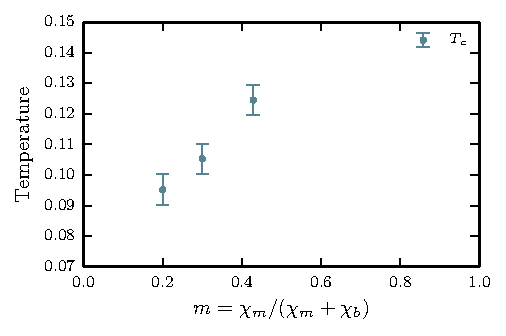
\includegraphics[width=\columnwidth]{CriticalTempVsMeasurementFraction.pdf}}}
\\
\vspace{-1.2\baselineskip}
\subfloat{\scalebox{1}{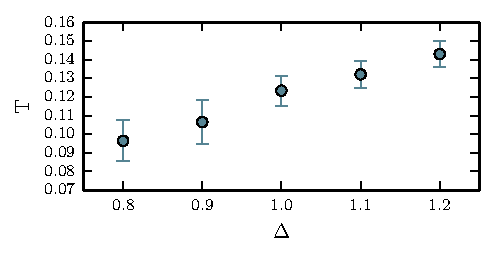
\includegraphics[width=\columnwidth]{CriticalTempVsDelta.pdf}}}  
\end{center}
\caption[justification=raggedright]{
Here we plot threshold temperatures as a function of measurement fraction, $m$, as well as the Hamiltonian energy scale $\Delta$ (see Eq. \ref{eq:isingham}).  At zero measurement fraction, the critical temperature is 0, and at unit measurement fraction, the critical temperature is $\sim 1$.
}
\label{fig:CriticalTempVsMeasurementFraction}
\end{figure}
%%%%%%%%%%%%%%%%%%%%%%


%************************EXPAND THIS PARAGRAPH A LITTLE

Finally, in Fig. \ref{fig:LifetimeVsTemperatureVsEnergy}, we plot the lifetime of the system in the presence of the protocol at various energy scales $\Delta$.  By contrasting Figures \ref{fig:LifetimeVsMeasurementFraction} and \ref{fig:LifetimeVsTemperatureVsEnergy}, one can deduce the relative benefits of error suppression via more measurement resources versus error suppression via hamiltonian engineering (i.e., a larger gap to excitation).



  %%%%%%%%%%%%%%%%%%%%%%
%%%%%%%%%%%%%%%%%%%%%%
\section{Generalization to Higher Dimension}
\label{sec:tc_alg}
%%%%%%%%%%%%%%%%%%%%%%

 In this section, we sketch how the algorithm presented in Sec. \ref{sec:ecc_alg} generalizes to a higher dimensional stabilizer quantum memory---the toric code.  Where the dynamics of the 1D Ising model are typified by one dimensional random walks of domain walls, the nonequilibrium dynamics of the toric code are driven by two dimensional random walks of ``quasiparticle'' excitations.  Consider the toric code hamiltonian:.
 \begin{align}
\Htc &= -\Delta_e \sum_v A_v -\Delta_m \sum_p B_p ,\label{eq:HTC}\\
A_v &\equiv \prod_{j \in v} \sigma_j^z,\quad B_p \equiv \prod_{j \in p} \sigma_j^x,\label{eq:AvBp}
\end{align}

where $v$ denotes the 4-spin vertices of the square lattice, and where and $p$ denotes the 4-qubit plaquettes on the edges of a 2D square lattice\needcite.
While domain wall excitations in the 1D ising model are associated with -1 eigenstates of the $\sigma_z^i \sigma_z^{i+1}$ stabilizers, quasiparticle excitations for the toric code are associated with -1 eigenstates of the $A_v$ and $B_p$ stabilizers as defined in Eq. \ref{eq:AvBp}.
 
 Broadly speaking, the algorithm is identical, but instead of having ``patches'' of measurement, there are measurement ``rails'', as indicated in \figref{fig:tc_fig}.  One such set of rails must exist for both types of excitations in the toric code---that is, one for the $B_p$ stabilizers, and another set of measurement rails for the $A_v$ stabilizers.  The error detection and correction can then be performed completely in parallel for both types of excitations, as they are independent.  ``Centering'' of defects on rails amounts to shift-swaping defects into the center of the measurement rail \red{Cite your previous paper?}.  We conjecture that a sparse measurement strategy with randomly placed measurement patches of fixed diameter might exist for sufficiently large and sufficiently cold systems.  However, the rail geometry of \figref{fig:tc_fig} is the simplest geometry that allows us to argue for a threshold temperature for the toric code, based on a generalization of the simple error model used for the Ising model in Sec. \ref{sec:threshold}.  The only difference between the upper bound to the expected scaling of the probability of uncorrectable errors in the toric code versus the expected scaling of the Ising model (i.e., Eq. \ref{eq:err_scaling}) is the prefactor becomes $\propto (L/\lambda)^2$ for the toric code instead of $L/\lambda$, where $L$ represents the linear dimension of the toric code.

\begin{figure}
\begin{center}
\scalebox{1}{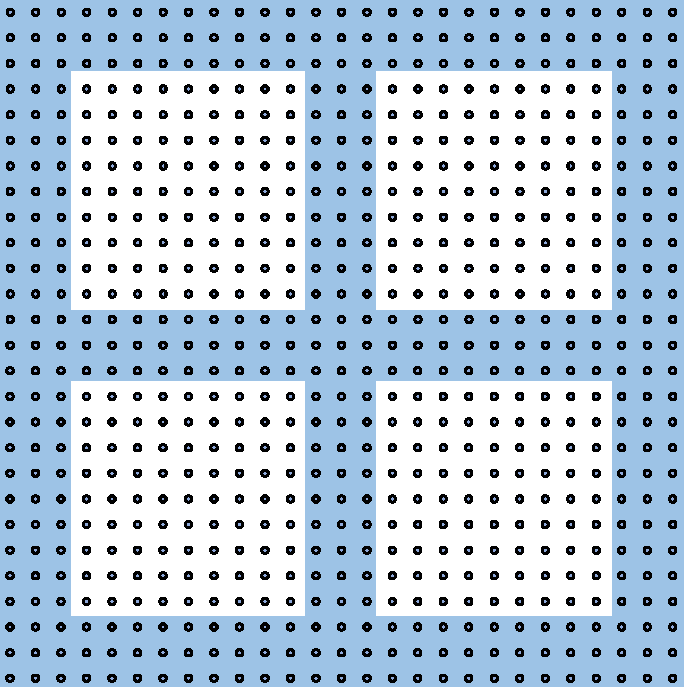
\includegraphics[width=1.0\columnwidth]{tc_fig_2.pdf}}
\end{center}
\caption{Here we sketch one possible $m=63/144$ (for a 12x12 unit cell) geometry for the measurement rails for a realization of our protocol.  More sparse geometries can be realized simply by moving the rails of measurement farther apart.  Measured sites are in light blue, and vertex locations for the toric code are circles.  Spin variables (not pictured) reside directly between neighboring vertices.}
\label{fig:tc_fig}
\end{figure}




 %%%%%%%%%%%%%%%%%%%%%%
%%%%%%%%%%%%%%%%%%%%%%
\section{Discussion}
\label{sec:discussion}
%%%%%%%%%%%%%%%%%%%%%%

We have provided numerical and theoretical evidence of a few-measurement error correction protocol for a stabilizer code with string-like excitations.  The primary technical innovation of our algorithm is a Bayesian decoding scheme for pairing defects based on partial information, sketched in Sec. \ref{sec:ecc_alg}. When combined with the measurement-free defect localization technique developed in Ref. \cite{Freeman2016}, this decoding scheme performs error correction efficiently and results in a stable quantum memory at temperatures lower than an empirically determined threshold temperature.  So long as an appropriate geometry of measurement devices is in place, and so long as defects undergo diffusive motion via coupling to a thermal bath, this scheme can be extended to higher dimensional stabilizer systems like the toric code, as demonstrated in Sec. \ref{sec:tc_alg}.

Our results complement what is known about decoders in the presence of \emph{noisy} measurements.  Figures \ref{fig:LifetimeVsMeasurementFraction} and \ref{fig:CriticalTempVsMeasurementFraction} demonstrate how a reduction in the measurement fraction in the lattice corresponds to a concomitant decrease in the threshold temperature, similar to how thresholds are known to be reduced when increasing the noise on measurements.

More fundamentally, our algorithm can be understood as an entropy reduction scheme.  Configurations that give rise to errors in the encoded subspace are exponentially suppressed as system size is made larger.  This is in contrast with ``energetic'' suppression---that is, suppression by widening the gap to excitations, $\Delta$ (or equivalently lowering the operating temperature).  This tradeoff between entropic and energetic contributions is depicted in Figures \ref{fig:LifetimeVsTemperatureVsEnergy} and \ref{fig:LifetimeVsMeasurementFraction}.  Depending on the resource requirements of a particular architecture, the threshold temperature can be tuned either by engineering a larger gap, $\Delta$, or by changing the number of measurements used.  In practice, this will depend on the lowest effective temperature available, the maximum measurement rate, as well as the practical difficulty of employing more measuring devices.



%%%%%%%%%%%%%%%%%%%%%%
\section{Acknowledgments}
This material is based upon work supported by DARPA under Grant No. 3854-UCB-AFOSR-0041 and by the National Science Foundation under Grants No. PIF-0803429 and No. CHE-1213141.  CDF was supported by the NSF Graduate Research Fellowship under Grant DGE-1106400 and by the DOE Office of Science Graduate Student Research (SCGSR) program under contract number DE‐SC0014664. MS was supported by the Laboratory Directed Research and Development program at Sandia National Laboratories.  Sandia National Laboratories is a multi-mission laboratory managed and operated by Sandia Corporation, a wholly owned subsidiary of Lockheed Martin Corporation, for the U.S. Department of Energy'�s National Nuclear Security Administration under contract DE-AC04-94AL85000. 

%%%%%%%%%%%%%%%%%%%%%%


\appendix
%%%%%%%%%%%%%%%%%%%%%%
\section{Bayesian Decoding for the Ising Model}
\label{sec:bayesdecoder}
%%%%%%%%%%%%%%%%%%%%%%

In this section, we provide further discussion of Eq. \ref{eq:bayes}, as well as analytic and numerical arguments for how it can be more simply approximated.

First, we decompose $P(d_1 : d_2)$ into two pieces: a combinatorial piece, and a dynamical piece.

For the combinatorial piece, note that a necessary condition for pairing to be possible is for both defects belonging to a pair to actually be measured.  That is, there might be a large number of measured defects ${d_1, d_2, ..., d_{n_m}}$, but the pairing defect for some of these defects might not be measured. Among those defects which are both measured, and which have their pair also measured, then the probability of selecting two defects that are a pair is simply the combinatorial factor $\frac{1}{\binom{N_{\rm{measured\ pair\ defects}}}{2}}$ where $N_{\rm{measured\ pair\ defects}}$ counts the average number of measured defects for which their pair is also measured.

The dynamical piece is the probability that $d_1$ and $d_2$ are defects whose pairs are also measured.  This probability depends on how quickly defects make excursions to measurement sites, as well as how quickly defects are being paired---either erroneously or correctly---by the protocol.  We can crudely lower bound this by taking the equilibrium defect distribution, and calculating the probability that a pair of defects lands on a measurement patch.  $\lambda_m / \lambda_t$ sites have measurement operators, thus $(\lambda_m / \lambda_t) L \gamma_+$ is an underestimate of the number of defects on measurement patches.  This is an underestimate because the protocol is actually more efficient at concentrating defects on measurement patches than equilibrium dynamics is.  Given $L \gamma_+$ pairs, this amounts to a binomial counting argument, and the expected number of measured pairs is simply $L \gamma_+ (\lambda_m / \lambda_t)^2$.  Thus, a lower bound to the equilibrium probability of two selected defects being a measured pair is simply $\frac{L \gamma_+(\lambda_m / \lambda_t)^2}{L \gamma_+} = (\lambda_m / \lambda_t)^2$.

As mentioned in Sec. \label{sec:bayes_prob_calc}, $P(d_1^{x_1,t_1}\wedge d_2^{x_2,t_2})$ is the probability that two defects are measured, one at $(x_1,t_1)$, and the other at $(x_2,t_2)$.  This can be decomposed:

\begin{align}
&P(d_1^{x_1,t_1}\wedge d_2^{x_2,t_2}) = \\ \notag
&P(d_1^{x_1,t_1} \wedge d_2^{x_2,t_2} | d_1:d_2) P(d_1 : d_2) + \\ \notag 
&P(d_1^{x_1,t_1} \wedge d_2^{x_2,t_2} | d_1\cancel{:}d_2) (1 - P(d_1 : d_2))
\end{align}

The first term is precisely Eq. \ref{eq:bayesformula}.  The second term represents the probability of two measurement events, conditioned on those events \emph{not} being part of a pair.  This is essentially the probability that two independent measurement events have occurred, which is approximately the probability that two independent creation events have occurred (assuming defects are measured suitably efficiently).  For a suitably large system at moderately low temperature, this probability can be estimated as $\propto \frac{|t_2-t_1|}{(L \gamma_+)^{-2}}:=\delta(L,T,\Delta t)$.

In practice, at low temperature for moderately sized systems, $P(d_1 : d_2)$ is very nearly $1$.  This arises from the low density of defects meaning that only rarely are there even a pair of defects in the system.  Of course, if system size is made sufficiently large, this bare probability will become diminished, but it is still the case that defects within a separation distance $2\sqrt{D |t_2 - t_1|}$ are, more often than not, a pair at low temperature.  For the same reason, $P(d_1^{x_1,t_1} \wedge d_2^{x_2,t_2} | d_1\cancel{:}d_2)$ is very nearly $0$ because this probability is roughly equivalent to the probability that two independent pair creation events have occurred, which is unlikely at low temperature and moderate system size.  Again, for sufficiently large systems this probability grows, but it is likewise the case that this probability is small for defects within a distance $2\sqrt{D |t_2 - t_1|}$.  Then, if we write $P(d_1 : d_2) = 1 - \epsilon(L,T)$, and perform some rearranging:

\begin{align}
\label{eq:bayes_simple}
&P(d_1:d_2 | d_1^{x_1,t_1} \wedge d_2^{x_2,t_2}) = \\ \notag
&\frac{1}{1+\frac{P(d_1^{x_1,t_1} \wedge d_2^{x_2,t_2} | d_1\cancel{:}d_2) \epsilon(L,T)}{P(d_1^{x_1,t_1} \wedge d_2^{x_2,t_2} | d_1:d_2) (1-\epsilon(T))}} \\ \notag
\geq &\frac{1}{1+\frac{\frac{\delta(L,T,\Delta t)}{1-\epsilon(L,T)}} {P(d_1^{x_1,t_1} \wedge d_2^{x_2,t_2} | d_1:d_2)}} \\ \notag
\approx &\frac{1}{1+\frac{\delta(L,T,\Delta t)}{P(d_1^{x_1,t_1} \wedge d_2^{x_2,t_2} | d_1:d_2)}}
\end{align}

Thus, only when $P(d_1^{x_1,t_1} \wedge d_2^{x_2,t_2} | d_1:d_2) << \delta(L,T,\Delta t)$ is this factor not equal to $1$.  This naturally occurs when comparing defects that are much farther apart than diffusive motion would usually allow.  For example: for a very large system, if one defect of a pair is measured at site $0$ and another defect belonging to another independent pair is measured at site $L/2$ shortly thereafter (compared to the timescale for defect motion), it is exceedingly unlikely for these two measured defects to be a pair because it's exponentially unlikely for such a long random excursion to occur.  In this way, the factor $P(d_1^{x_1,t_1} \wedge d_2^{x_2,t_2} | d_1:d_2)$  serves as an indicator function which answers the question, ``Could these two defects have arisen from a random walk starting in the same place?''.  The factor $\delta(L,T,\Delta t)$ sets the cutoff for a plausible excursion---i.e., when the error function is much less than this term, the denominator of \ref{eq:bayes_simple} blows up, and the probability of performing that fusion is essentially zero.

In practice, the precise details of these additional factors arising from Bayes theorem aren't too important for the protocol to function, and we find that using the conditional probability $P(d_1^{x_1,t_1} \wedge d_2^{x_2,t_2} | d_1:d_2)$ itself as a proxy for the full expression from Bayes theorem is sufficient to reliably correct errors.  We provide some heuristic comparisons of different decoding schemes in appendix TODOGOHERE.



\bibliography{manuscript_TC_2}

\end{document}